% load relevant packages
\documentclass[11pt,a4paper]{article}
\usepackage[hyperref]{acl2020}
\usepackage{times}
\usepackage{lipsum}
\usepackage{amsmath}
\usepackage{amssymb}
\usepackage{mathtools}
\usepackage{latexsym}
\usepackage{graphicx}
\graphicspath{{../../img/}}
\renewcommand{\UrlFont}{\ttfamily\small}
\usepackage{microtype}
\aclfinalcopy
%\setlength\titlebox{5cm}
\newcommand\BibTeX{B\textsc{ib}\TeX}

% administrative details
\title{Investigating the isometric properties of Neural Machine Translation models on binary semantic-equivalence spaces}
\author{Atreya Shankar \\
  Cognitive Systems, University of Potsdam \\
  Department of Computational Linguistics, University of Zürich \\
  \texttt{atreya.shankar@\{uni-potsdam.de,uzh.ch\}}}
\date{\today}

% start document
\begin{document}

% produce title
\maketitle

% abstract
\begin{abstract}
  \textit{Isometry} is defined mathematically as a distance-preserving transformation between two metric spaces. In this research, we hypothesize that well-performing Neural Machine Translation (NMT) models function approximately isometrically on semantic metric spaces. That is to say, if two sentences are semantically equivalent on the source side, they should remain semantically equivalent after translation on the target side. We begin by utilizing two NMT models of varying performance to translate semantically-equivalent paraphrases based off WMT19 test data references. In order to quantify and simplify the notion of a semantic metric space, we treat it as a probabilistic binary semantic-equivalence space indicating either semantic equality or inequality; achieved by fine-tuning three transformer-based language models on Google's PAWS-X paraphrase detection task. By using the paraphrase detection outputs, we investigate the frequency and composition of semantically isometric behaviour in the NMT models' inputs and outputs.
\end{abstract}

% body
\section{Introduction}

\textit{Isometry} is defined mathematically as a distance-preserving transformation between two metric spaces \cite{coxeter1961introduction}. In this research, we view Neural Machine Translation (NMT) models from the perspective of semantic isometry and hypothesize that well-performing NMT models function approximately isometrically on semantic metric spaces. That is to say, if two sentences are semantically equivalent on the source side, they should remain semantically equivalent after translation on the target side given a well-performing NMT model. A simplified illustration of isometry in higher dimensional functional spaces can be seen in Figure \ref{isometry_visual}.

In order to conduct our investigation, we start by acquiring semantically equivalent paraphrases of WMT19 legacy and additional test references from \citet{freitag-bleu-paraphrase-references-2020} for \texttt{en$\rightarrow$de}. Next, we utilize two NMT models of varying performance, specifically the SOTA FAIR's WMT19 winning single transformer \cite{ng2019facebook} and the non-SOTA Scaling NMT WMT16 Transformer \cite{ott2018scaling}, in order to translate the aforementioned paraphrases in the \texttt{de$\rightarrow$en} translation direction. We use the former model pre-trained from \texttt{fairseq} \cite{ott2019fairseq} and train the latter model from scratch.

\begin{figure}
  \centering
  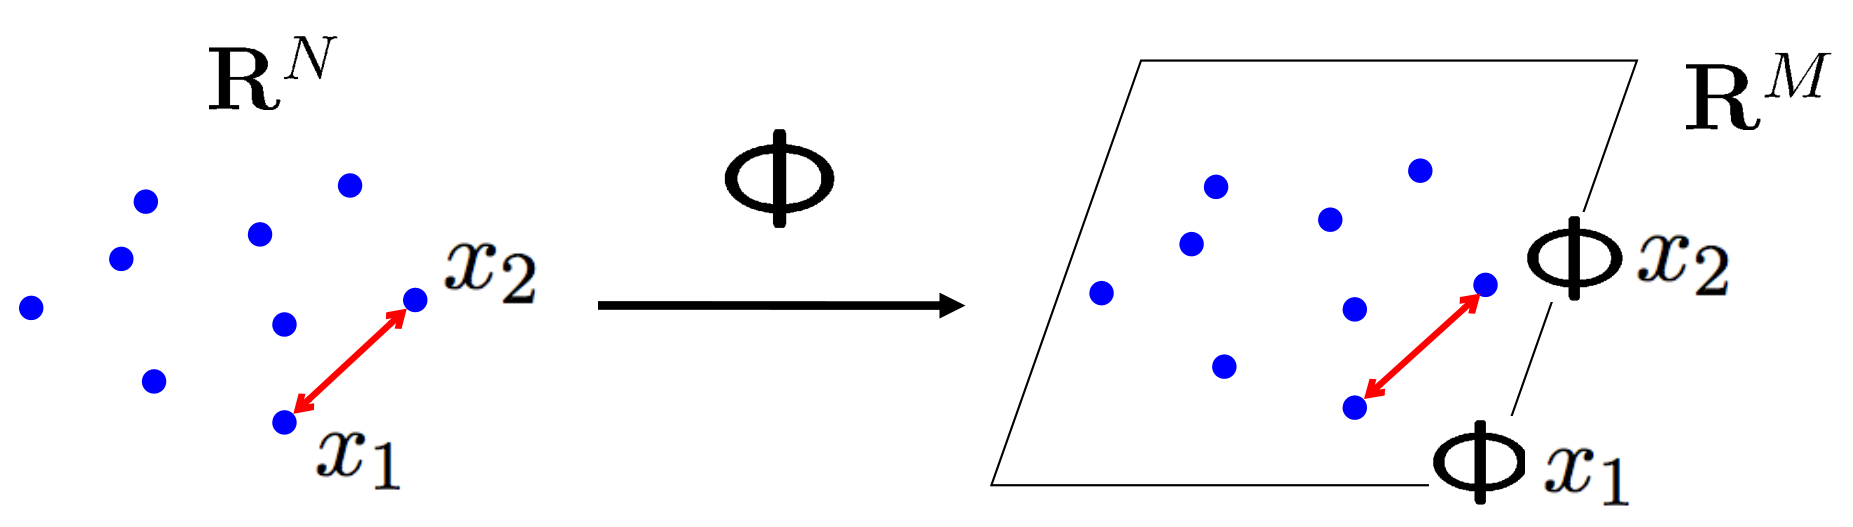
\includegraphics[trim={1.0cm 0cm 0cm 1.0cm},clip,width=0.52\textwidth]{isometry_visualized.png}
  \caption{Illustration of isometry in higher dimensional functional transformations \citep{Hegde-Numax}}
  \label{isometry_visual}
\end{figure}

Next, we utilize three well-performing paraphrase detection models to approximate isometry in the NMT models' translations. These paraphrase detection models are based off mBERT\textsubscript{Base} \cite{devlin-etal-2019-bert}, XLM-R\textsubscript{Base} \cite{conneau2019unsupervised} and XLM-R\textsubscript{Large} \cite{conneau2019unsupervised} pre-trained multilingual language models; which are correspondingly fine-tuned on Google's PAWS-X paraphrase detection task \cite{pawsx2019emnlp, hu2020xtreme}.
 
Using the outputs of the paraphrase detection models, we finally investigate the frequency and composition of semantically isometric behaviour in the NMT models' inputs and outputs. We document our investigation and provide relevant source code in our public GitHub repository\footnote{\url{https://github.com/atreyasha/semantic-isometry-nmt}}.

% 1. Introduction
% TODO add post-paper contributions as concretely as possible -> add into abstract as well
% TODO state expectations more concretely here and in abstract
% TODO state hypothesis more clearly that isometry is positively correlated with general performance of a model -> perhaps show this statistically where possible with appropriate statistical test
% TODO think of title and how this links up with everything -> change it to reflect content of paper if necessary
% TODO make abstract more similar to introduction where possible
% TODO add github repository and any other important links inside paper
% look up fairseq API and whether this is correct usage
% fix "based off" and change to something else to get diversity

\section{Isometry and approximations}

The concept of isometry in the context of semantic metric spaces can be \textit{exactly} expressed as follows; where $s_i \in \mathbb{R}^{V \times N}$ refers to an input sentence's tokenized matrix-form for vocabulary size $V$ and sentence length $N$, $f: \mathbb{R}^{V \times N} \to \mathbb{R}^{V' \times N'}$ refers to the NMT model's inference function and $D_L: \mathbb{R}^{V \times 2N} \to \mathbb{R}_+$ refers to a semantic distance metric function for language $L$ corresponding to the language of the respective sentences:

\begin{equation}  
  \label{exact_isometry_eqn}
  D_Y(f(s_1),f(s_2)) = D_X(s_1,s_2)
\end{equation}

While elegant, this representation of isometry and a semantic distance metric is problematic. Firstly, exact isometry might not be a practical condition to achieve given real-life data instances with stochastic noise. Next, constructing continuous semantic metric spaces from discrete textual data is a difficult task and is in itself a developing field of research \cite{cer2017semeval}.

\paragraph{Approximate isometry:} To address the first issue, we loosen the constraints of exact isometry to \textit{approximate} isometry:

\begin{equation} 
  \label{approx_isometry_eqn}
  D_Y(f(s_1),f(s_2)) \approx D_X(s_1,s_2) 
\end{equation}

With this approximation, we can simplify the isometric relationship further into a binary semantic-equivalence function $S_L: \mathbb{R}^{V \times 2N} \to \{0,1\}$, which compresses semantic distance metrics to semantic equality ($S_L=1$) or inequality ($S_L=0$) depending on some variable threshold $\delta_L \in \mathbb{R}_+$:

\begin{equation}
  \label{bounded_isometry_eqn}
  S_L(s_1,s_2) =
  \begin{cases}
    1, &D_L(s_1,s_2) \leq \delta_L \\
    0, &D_L(s_1,s_2) > \delta_L
  \end{cases}
\end{equation}

It is worth noting that the formulation in $S_L$ is more meaningful for inferring isometry from semantic equality than from semantic inequality, due to the presence of a tighter bound for the former than the latter.

\paragraph{Probabilistic semantic-equivalence spaces:} To address the second issue, we effectively delegate away the actual computation of a semantic distance metric and convert this into a probabilistic process; with a new definition for $S_L$ below given a probability threshold $\epsilon$ with a typical value of 0.5. This reformulation allows for the utility of statistical paraphrase detection models without explicit computation of semantic metric spaces. 

\begin{equation}
  \label{bounded_isometry_probability_eqn}
  S_L(s_1,s_2) =
  \begin{cases}
    1, &P\big(D_L(s_1,s_2) \leq \delta_L\big) \geq \epsilon \\
    0, &P\big(D_L(s_1,s_2) \leq \delta_L\big) < \epsilon
  \end{cases}
\end{equation}

With the aforementioned simplifications, we now re-write our equation for approximate isometry as follows:

\begin{equation}  
  \label{exact_approx_isometry_eqn}
  S_Y(f(s_1),f(s_2)) = S_X(s_1,s_2)
\end{equation}

% 2. Motivation (or more thematic title)
% TODO extrapolate respective changes from here to all sections with terminology
% TODO consider changing paraphrase score to distance metric -> depends on how the research is presented
% TODO consider changing name to semantic-similarity or paraphrase-detection space -> think of how to not make this misleading and how to not confuse discete and continuous semantic spaces
% TODO consider calling analysis semantic-equivalence-step functions or probabilistic semantic-equivalence, or binary might be good enough -> consider getting rid of metric spaces if they are not useful
% think more about whether to include or exclude adversarial term since this might be a grey area -> qualify various means of being adversarial ie. targetted through model or perhaps just an intention

\section{Related work}

Based on a survey of recent literature in Natural Language Processing (NLP) and NMT, we were unable to find explicitly similar studies to our research. However, we would argue that the closest field in NLP to this research would be \textit{adversarial paraphrasing}.

\citet{michel2019evaluation} describes adversarial paraphrasing in the purview of machine translation as constructing paraphrases that are \textit{``meaning preserving on the source-side, but meaning-destroying on the target-side''}. For the sake of comparison, we would mildly \textit{paraphrase} this description of adversarial paraphrasing to \textit{``the process of perturbing an input sentence such that it is semantically equivalent on the source-side, but semantically inequivalent on the target-side"}.

In this sense, the study of adversarial paraphrasing in machine translation could be interpreted as a targetted probe into semantic \textit{anisometry} of NMT models, compared to our research which would be an untargetted probe into semantic isometry of NMT models. Therefore adversarial paraphrasing, while having the opposite intent, is still highly similar to our research.

\paragraph{\citet{michel2019evaluation}:} This research lays out the framework for evaluating adversarial perturbations in sequence-to-sequence models. Additonally, this research compared three automatic sequence evaluation metrics, specifically \texttt{BLEU} \cite{papineni2002bleu}, \texttt{METEOR} \cite{denkowski2014meteor} and \texttt{chrF} \cite{popovic2015chrf}, against human judgment for evaluating semantic similarity. Results from their experiments showed that \texttt{chrF} correlates best out of the three similarity metrics with human judgment for semantic similarity detection. We utilize this finding in later parts of our study and attempt to compare the outputs of our paraphrase detection models with respective \texttt{chrF} scores.

\paragraph{\citet{fadaee2020unreasonable}:} This research lays out a simple framework for constructing adversarial paraphrases through logical operations such as word insertion/deletion and numerical/gender substitution. The research correspondingly showed that such minor modifications could lead to disproportionately larger changes in translation outputs; thereby showing an adversarial effect. This research ultimately claimed that modern NMT models are generally \textit{volatile}, or vulnerable, to targetted adversarial attacks. We attempt to compare this claim with our findings in later parts of this study. 

% 3. Related work
% TODO consider removing comparisons to own study at the end of related work descriptions
% much work has been done on paraphrase detection but not neccessarily linking this directly to translation models -> would be an interesting link to NMT model evaluation

\section{Experimental setup}

\subsection{Data sets}

Below we describe the key data sets that we were used in our research.

\subsubsection{WMT19 en-de references and corresponding paraphrases}

\citet{freitag-bleu-paraphrase-references-2020} builds on the premise that while automatic evaluation metrics, such as \texttt{BLEU}, are important for NMT model evaluation; the presence of diverse translation references is also critical. Motivated by the observation that typical references show poor diversity, \citet{freitag-bleu-paraphrase-references-2020} focuses on two goals; namely creating additional high quality WMT19 test references, as well as paraphrasing both existing (or legacy) and additional WMT19 test references in the \texttt{en$\rightarrow$de} translation direction.

These services were ultimately rendered by a professional translation service using different sets of linguists for different tasks to reduce systematic bias. While these additional references serve the purpose of diversifying evaluation references, we see them as a source of high-quality semantically equivalent paraphrases with varied lexical and syntactical features. We therefore use these additional references as our input paraphrase sentences to investigate semantic isometry. Below are the key resulting data sets for \texttt{en$\rightarrow$de} that were used in our research.

\paragraph{WMT19 legacy test references:} This refers to the existing \texttt{newstest2019} translation references without any additional references or paraphrasing. For abbrevation purposes, we refer to this data set as \texttt{WMT}. 

\paragraph{WMT19 additional test references:} This refers to additional references produced as a result of \citet{freitag-bleu-paraphrase-references-2020}. For abbrevation purposes, we refer to this data set as \texttt{AR}. 

\paragraph{WMT19 legacy test paraphrased references:} This refers to the paraphrased version of the existing \texttt{newstest2019} translation references produced as a result of \citet{freitag-bleu-paraphrase-references-2020}. For abbrevation purposes, we refer to this data set as \texttt{WMT.p}. 

\paragraph{WMT19 additional test paraphrased references:}This refers to the paraphrased version of the additional translation references produced as a result of \citet{freitag-bleu-paraphrase-references-2020}. For abbrevation purposes, we refer to this data set as \texttt{AR.p}.

For brevity, we further simplify the aforementioned data sets as follows:

\vspace{-10pt}
\begin{align}
  \text{WMT19 Legacy} &= \{\text{WMT} \cup \text{WMT.p} \} \\
  \text{WMT19 AR} &= \{\text{AR} \cup \text{AR.p} \}
\end{align}

\subsubsection{PAWS-X}

PAWS-X is a cross-lingual adversarial data set for paraphrase identification released by Google Research \citep{pawsx2019emnlp}. PAWS-X stems originally from the PAWS data set released by \citet{zhang2019paws} which is an abbreviation for \textbf{P}araphrase \textbf{A}dversaries from \textbf{W}ord \textbf{S}crambling.

The original motivation behind the PAWS data set was that existing paraphrase detection data sets lacked non-paraphrase sentence pairs with high lexical overlap. The PAWS data set was therefore released to drive progress in creating models that utilize fine-grained structure and context of sentence pairs.

\begin{figure*}
  \centering 
  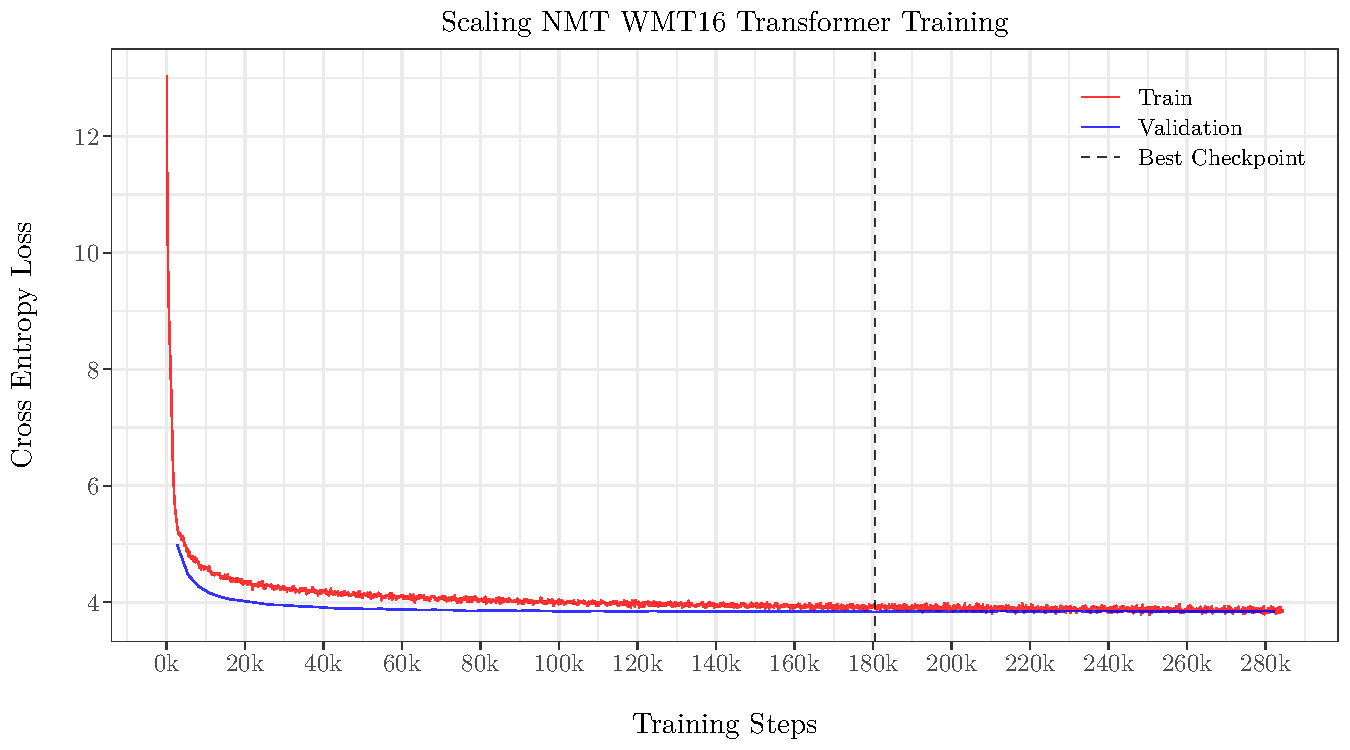
\includegraphics[trim={0cm 0cm 0cm 0cm},clip,width=\textwidth]{transformer_nmt_evolution.pdf}
  \caption{Training and validation cross entropy loss for Scaling NMT WMT16 Transformer}
  \label{transformer_nmt_evolution}
\end{figure*}

The PAWS data set contains 108,463 paraphrase and non-paraphrase sentence pairs with high lexical overlap. These sentence pairs were bulk sourced from Wikipedia and Quora Question Pairs; followed by controlled word swapping and back translation to create challenging sentence pairs for paraphrase detection. The generated sentence pairs were finally evaluated for fluency and general quality by human raters.

As noted in \citet{pawsx2019emnlp}, one limitation of adversarially generated data sets such as PAWS is their pre-dominant focus on the English language. In order to address this issue, \citet{pawsx2019emnlp} released PAWS-X; which consists of 23,659 human translated evaluation sentence pairs and 296,406 machine-translated training sentence pairs derived from the Wikipedia subset of the original PAWS data set. These sentence pairs were translated from English to six typologically distinct languages; namely French, Spanish, German, Chinese, Japanese and Korean.

The release of PAWS-X provides many advantages to the field of NLP, particularly the creation of a new benchmark to promote research in multilingual and zero-shot paraphrase detection. This can already be seen by the incorporation of PAWS-X into Google's recent Cross-lingual TRansfer Evaluation of Multilingual Encoders (XTREME) benchmark system \cite{hu2020xtreme}.

\subsubsection{WMT16 de-en}

In this study, we replicate a non-SOTA NMT model from scratch based off the Scaling NMT WMT16 workflow \cite{ott2018scaling}. While the original implementation in \citet{ott2018scaling} is based on the \texttt{en$\rightarrow$de} translation direction, our implementation trains a NMT model in the reverse translation direction; specifically \texttt{de$\rightarrow$en}.

For this, we use WMT16 \texttt{de$\rightarrow$en} training data with 4.5M sentence pairs, \texttt{newstest2013} as our validation set and \texttt{newstest2014} as our test set. We utilize a vocabulary of 32K symbols based off a joint source and target byte-pair encoding (BPE; \citealt{sennrich2015neural}).   

% 4.1. Data sets
% TODO check consistent spelling of data sets across paper
% TODO be clear about translation direction -> check for consistency throughout paper on direction
% explain why AR was used, to provide additional paraphrases on top of legacy data since legacy WMT19 test data was shown to be poorly sourced -> talk about paraphrasing done very strongly which is why some were zeros on the source side already
% bring up actual examples of paraphrases and detection tasks -> to give some perspective

\subsection{Models}

Below we describe the key models that were used in our research.

\subsubsection{FAIR WMT19 Transformer}

We utilize FAIR's winning WMT19 single Transformer model as our SOTA NMT model. Focusing particularly on the \texttt{de$\rightarrow$en} translation direction, the FAIR WMT19 Transformer was the top performing model in WMT19 with a SacreBLEU score of 40.8.

As per \citet{ng2019facebook}, the key factors that led to SOTA performance include \texttt{langid} filtering of crawled bitext data, large-scale back translation as a form of data augmentation and noisy channel model reranking. We utilized this model directly from the \texttt{fairseq} API \cite{ott2019fairseq}. 

\subsubsection{Scaling NMT WMT16 Transformer}

We replicate the Scaling NMT WMT16 Transformer based on \citet{ott2018scaling} by training it from scratch. However, we swap the translation direction from \texttt{en$\rightarrow$de} to \texttt{de$\rightarrow$en}; such that we can ultimately use this model to translate WMT19 paraphrases from \texttt{de$\rightarrow$en}. We intentionally choose this workflow since it would produce a non-SOTA transformer which would be useful for us downstream to introduce performance-dependent variance in the translation of WMT19 paraphrases.

\begin{figure*}
  \centering 
  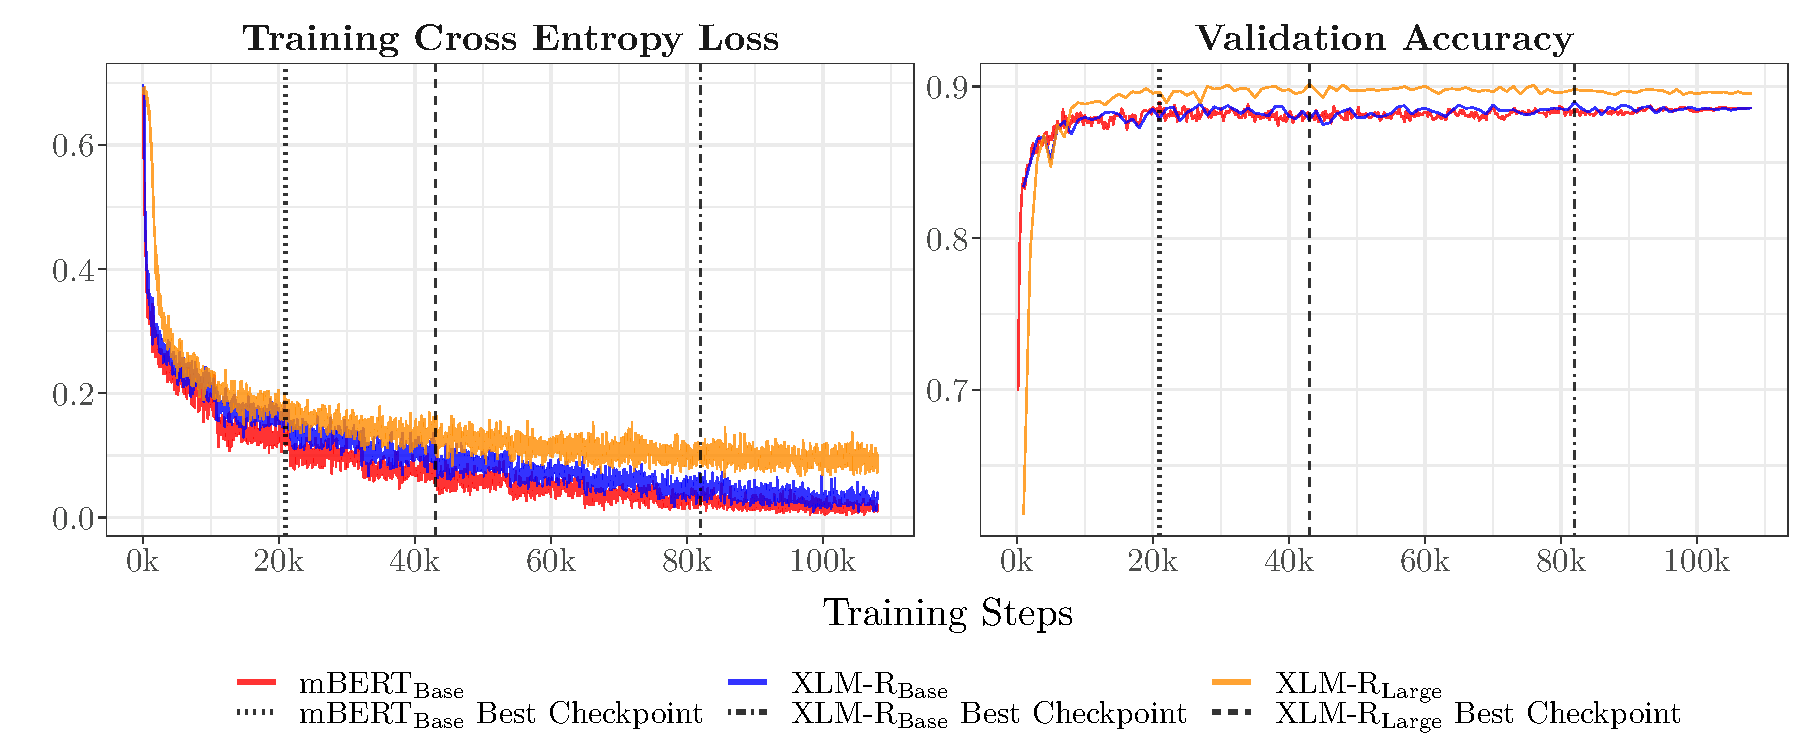
\includegraphics[trim={0.7cm 0cm 0cm 0cm},clip,width=\textwidth]{paraphrase_detection_models_evolution.pdf}
  \caption{Training loss and validation accuracy w.r.t. training steps for paraphrase detection models}
  \label{paraphrase_detection_model_evolution}
\end{figure*}

Besides the aforementioned modification, we follow the same setup as per \citet{ott2018scaling}. Specifically, we use a ``big'' transformer model based off \citet{vaswani2017attention}; with 6 blocks in the encoder and decoder networks. This model has a total of 210M parameters.

During training, we apply dropout \cite{srivastava2014dropout} with probability 0.3 and utilize the Adam optimizer \cite{kingma2014adam} with $\beta_1 = 0.90$ and $\beta_2=0.98$. We use a learning rate schedule where the learning rate increases linearly for 4,000 steps from 1e-7 until 1e-3. The learning rate then decays proportionally to the inverse square root of the number of training steps. We utilize label smoothing with weight 0.1 for the uniform prior distribution over the vocabulary \cite{pereyra2017regularizing}. We use large batch sizes with the maximum number of tokens per batch being 7168. Furthermore, we apply gradient accumulation for 8 steps before updating the model; which is known as \texttt{update-freq} in the \texttt{fairseq} API. We also exploit \texttt{fairseq}'s half precision floating point (FP16) functionality for more efficient training.

Finally, we train this model for 6 days on a single NVIDIA Tesla-V100 16GB GPU. During training, we monitor the validation loss and enable checkpoint-saving for the best performing checkpoint on the validation set. We train the model up until $\sim$285K updates.

Our best performing checkpoint was saved at $\sim$180K updates as seen in Figure \ref{transformer_nmt_evolution}. For evaluation on the test set, we utilize beam search with a beam width of 5. Our final Scaling NMT WMT16 Transformer achieved a SacreBLEU score\footnote{\footnotesize SacreBLEU signature:\\BLEU+case.mixed+lang.de$\nobreakdash$en+numrefs.1+smooth.exp+\\test.wmt14/full+tok.13a+version.1.4.12} of 31.0 on the \texttt{newstest2014} test set.

\subsubsection{Paraphrase detection models}

As noted in equation \ref{bounded_isometry_probability_eqn}, paraphrase detection models are useful in computing probabilistic semantic-equivalence spaces, or otherwise the $S_L$ function. We follow a similar framework as that detailed in Google's XTREME benchmark \cite{hu2020xtreme} and fine-tune pre-trained multilingual transformer language models on the PAWS-X paraphrase detection task. We focus specifically on three multilingual transformer language models, specifically mBERT\textsubscript{Base} (104 languages; 172M parameters; \citealt{devlin-etal-2019-bert}), XLM-R\textsubscript{Base} (100 languages; 270M parameters; \citealt{conneau2019unsupervised}) and XLM-R\textsubscript{Large} (100 languages; 550M parameters; \citealt{conneau2019unsupervised}) using HuggingFace's \texttt{transformers} library \cite{Wolf2019HuggingFacesTS} with model variants optimized for sequence classification.

While our implementation is similar to that of Google's XTREME benchmark, we modify some aspects of the workflow to suit our needs. Most importantly, we fine-tune our multilingual language models on PAWS-X training data from all 7 languages instead of only English in order to reap the benefits of diverse multilingual data.

\begin{table}
  \centering
  \begin{tabular}{llll}
    \hline
    \textbf{Language} & \textbf{mBERT\textsubscript{B}} & \textbf{XLM-R\textsubscript{B}} & \textbf{XLM-R\textsubscript{L}} \\
    \hline
    en & 0.940 & 0.946 & 0.960 \\
    de & 0.898 & 0.900 & 0.912 \\
    es & 0.908 & 0.922 & 0.928 \\
    fr & 0.922 & 0.917 & 0.933 \\
    ja & 0.836 & 0.836 & 0.859 \\
    ko & 0.841 & 0.847 & 0.870 \\
    zh & 0.854 & 0.861 & 0.876 \\
    \hline \hline
    $\mu$ & 0.886 & 0.890 & \textbf{0.906} \\
    \hline
  \end{tabular} 
  \caption{Language-specific summary of macro-F\textsubscript{1} scores of paraphrase detection models on the PAWS-X test set; B and L refer to base and large respectively}
  \label{pawsx_score_breakdown}
\end{table}

For all models, we enforce a maximum sequence length of 128 tokens since PAWS-X sentence pairs generally fit it into this range. We train all models for 10 epochs or $\sim$110K updates with a global batch size of 32. We also use a linearly decaying learning rate schedule without warmup steps. Lastly, we monitor accuracy on the PAWS-X validation set for all languages in order to determine the best performing checkpoint.

Specific to mBERT\textsubscript{Base} and XLM-R\textsubscript{Base}, we use a batch size of 32 without gradient accumulation and an initial learning rate of 2e-5. As for XLM-R\textsubscript{Large}, we use an initial learning rate of 1e-6 and local batch size of 8 with 4 gradient accumulation steps to curb GPU out-of-memory (OOM) issues.

We fine-tune mBERT\textsubscript{Base}, XLM-R\textsubscript{Base} and XLM-R\textsubscript{Large} for 14 hours, 15 hours and 2.5 days on a single NVIDIA Gefore GTX 1080 Ti-12GB GPU respectively. The best checkpoints are achieved and saved at $\sim$20K, $\sim$80K and $\sim$40K updates respectively, as seen in Figure \ref{paraphrase_detection_model_evolution}.

As seen in Table \ref{pawsx_score_breakdown}, all three models perform well especially on our target languages of \texttt{en} and \texttt{de}. Overall, the best performing model on the PAWS-X test set is XLM-R\textsubscript{Large} with a macro-F\textsubscript{1} of 0.906.

\subsection{Evaluation protocols}

% 4.3 Evaluation protocols
% TODO motivate why we use multiple models instead of one
% TODO change score labels with P/S -> define in paper
% TODO use some logical symbols to show mode function and other interesting characteristics
% TODO list out protocols for evaluation
% TODO state expectations about outcomes, some basic ideas
% TODO consider refining and synchronizing model names as was done with data -> update plots
% TODO define probability threshold epsilon in paper when necessary
% go into techniques used, how isometric properties would be determined -> would need to be thought of more
% correlations to chrF to compare with Michel et al. 2019 -> how this would be done

% 5. Results (facts)
% bring in main charts and show results
% correlations to chrF to compare with Michel et al. 2019
% keep it simple and facts-ish
% show tables with chrF inter-comparisons and possibly BLEU -> try to enumerate as many results as possible -> mention why this was done to simulate commutivity of similarity metrics

% 6. Discussion (interpretation & comparisons)
% go into some examples for interpretations
% look into statistical test between isometry and model performance in general
% hard to prove this unless we re-train the SOTA model without backtranslation -> possible future task
% contributions to Michel et al. 2019 analysis where possible
% go into discussion regarding chrF and semantic equality -> try to make statistical claims where possible and use statistical tests to show that chrF is only useful for edge cases and otherwise not really -> use plots where possible and otherwise add abc annotations via ggplot if necessary
% explain that papers like volatility one might be making claims based on weaker models that could be fixed by using larger models with better training -> hard to say exactly but based on our paraphrases which are non-adversarial and non-targetted, this seems to be the case but also no hard conclusion -> depends on also which model they used
% list hypotheses and how some were refuted by results
% make less confident conclusion on relationship between back-translation and translation consistency -> could also be linked to other differences between models
% there are many possible contributions to better performance compared to non-SOTA -> could be langids to help prevent language mixing (observed in non-SOTA), could be backtranslation for syntactical and lexical diversity which contributes to paraphrase robustness
% provide some minor criticisms where appropriate -> such as some sentences being over-paraphrased

% 7. Conclusions
% main conclusions from this on isometry -> could be linked either to test data better fitting to WMT19 or otherwise massive backtranslation which provides some regularizing effect for FAIR SOTA model
% summarize everything and list contributions of this paper

% 8. Recommendations
% WMT16 transformer optimized for short sentences -> might make comparison also not good -> WMT16 vs. WMT19 issue which is a limitation of this research -> better to have used a WMT19 variant which was less performant
% paraphrase detection models are not commutative -> not logical in that sense -> maybe cosine similarity comparisons could help but might affect performance
% describe processes that worked and did not work -> talk about all the hurdles and show some bad examples when they occurred -> summarized below in logs
% limitation of system is that WMT19 might be more advantageous to FAIR model, which might have led to bad results in general for non-SOTA model
% Criticism of using WMT19 model is that it may be biased towards the WMT19 test set compared to the model trained on WMT16

% Post-paper formatting:
% do thorough language check on overleaf or otherwise to ensure proper grammar and spelling
% consider adding page numbers for easier reading

\clearpage
% references
\bibliography{bibtex}
\bibliographystyle{acl_natbib}

% end document
\end{document}